\documentclass{csbeamer}

\usepackage{dsfont}
\usepackage{amsmath}
\usepackage{amssymb}
\usepackage{algorithm}
\usepackage{algpseudocode}
\usepackage{pgfplots}
\usepackage{colortbl}
\usepackage{xcolor}
\pgfplotsset{compat=1.18}

% Add custom color definitions for Eligibility Traces
\definecolor{etmain}{HTML}{7B1FA2}
\definecolor{etaccent}{HTML}{FF5722}
\definecolor{etlight}{HTML}{BA68C8}
\definecolor{etsecondary}{HTML}{3F51B5}
\definecolor{eteval}{HTML}{2E7D32}
\definecolor{etimprove}{HTML}{E91E63}
\definecolor{etvalue}{HTML}{FF9800}
\definecolor{etpolicy}{HTML}{795548}
\definecolor{ettrace}{HTML}{9C27B0}
\definecolor{etlambda}{HTML}{1976D2}
\definecolor{etactivity}{HTML}{00BCD4}
\definecolor{eterror}{HTML}{D32F2F}
\definecolor{etbackward}{HTML}{4CAF50}

\university{St. Francis Xavier University}
\department{Department of Computer Science}
\course{CSCI-531 - Reinforcement Learning}
\courseshort{CSCI-531 - RL}
\term{Fall 2025}
\author{Dr. Jean-Alexis Delamer}

\title{Eligibility Traces}

\begin{document}

\frame{\titlepage}

% Section: Introduction
\section{Introduction}

\subsection{Bridging Monte Carlo and TD}

\begin{frame}
    \frametitle{The Unifying Mechanism}

    \begin{block}<1->{Two Methods We've Seen}
        \begin{itemize}
            \item<1-> \textcolor{etmain}{\textbf{Monte Carlo Methods}}: Wait for complete episodes
            \item<2-> \textcolor{etaccent}{\textbf{Temporal-Difference Methods}}: Learn at each step
        \end{itemize}
    \end{block}

    \begin{block}<3->{Activity}
        \textcolor{etactivity}{\textbf{What is the main difference between Monte Carlo and TD methods?}}
    \end{block}

    \begin{block}<4->{Answer}
        \begin{itemize}
            \item<4-> \textbf{Monte Carlo}: Uses actual returns, no bootstrapping
            \item<5-> \textbf{TD}: Uses estimated returns, bootstrapping from current estimates
            \item<6-> \textbf{Trade-off}: Bias vs. variance, speed vs. accuracy
        \end{itemize}
    \end{block}

    \begin{block}<7->{Enter Eligibility Traces}
        \textcolor{etmain}{\textbf{Eligibility traces}} provide a mechanism that \textcolor{ettrace}{\textbf{unifies}} both methods!
    \end{block}
\end{frame}

\begin{frame}
    \frametitle{What Are Eligibility Traces?}

    \begin{block}<1->{Key Concept}
        \textcolor{etmain}{\textbf{Eligibility traces}} are a short-term memory mechanism that bridges MC and TD methods.
    \end{block}

    \begin{block}<2->{The Mechanism}
        \begin{itemize}
            \item<2-> \textcolor{ettrace}{\textbf{Eligibility trace vector}}: $\mathbf{z}_t \in \mathbb{R}^d$
            \item<3-> Parallel to the weight vector $\mathbf{w}_t$
            \item<4-> \textcolor{etlambda}{\textbf{Trace-decay parameter}}: $\lambda \in [0,1]$
        \end{itemize}
    \end{block}

    \begin{block}<5->{How It Works}
        \begin{enumerate}
            \item<5-> When a component of $\mathbf{w}_t$ is used to estimate a value
            \item<6-> The corresponding component of $\mathbf{z}_t$ is \textcolor{etaccent}{\textbf{increased}}
            \item<7-> Then it starts to \textcolor{etlight}{\textbf{fade away}}
        \end{enumerate}
    \end{block}

    \begin{block}<8->{Intuition}
        \textcolor{etsecondary}{\textit{"Which states were recently visited and should get credit for the current reward?"}}
    \end{block}
\end{frame}

\begin{frame}
    \frametitle{Advantages of Eligibility Traces}

    \begin{block}<1->{Benefits Over Previous Methods}
        \begin{itemize}
            \item<1-> \textcolor{eteval}{\textbf{Single error signal}}: Only one TD error needed for updates
            \item<2-> \textcolor{etimprove}{\textbf{Online learning}}: Updates happen at each step
            \item<3-> \textcolor{etbackward}{\textbf{Backward view}}: Past states get immediate credit
            \item<4-> \textcolor{etvalue}{\textbf{Computational efficiency}}: No need to store entire trajectories
        \end{itemize}
    \end{block}

    \begin{block}<5->{The Credit Assignment Problem}
        \begin{itemize}
            \item<5-> \textbf{Problem}: Which past actions led to current reward?
            \item<6-> \textbf{Solution}: Traces remember recent state visits
            \item<7-> More recent visits get \textcolor{ettrace}{\textbf{more credit}}
        \end{itemize}
    \end{block}

    \begin{block}<8->{Key Insight}
        \textcolor{etmain}{\textbf{Eligibility traces allow us to learn from every step while considering the full trajectory!}}
    \end{block}
\end{frame}

% Section: Lambda Returns
\section{The $\lambda$-Return}

\subsection{N-Step Returns Revisited}

\begin{frame}
    \frametitle{Building Up to $\lambda$-Returns}

    \begin{block}<1->{Recall: N-Step Returns}
        \begin{equation}
            G_{t:t+n} = r_{t+1} + \gamma r_{t+2} + \cdots + \gamma^{n-1}r_{t+n} + \gamma^n\hat{v}(s_{t+n}, \mathbf{w}_{t+n-1})
        \end{equation}
        where $0 \leq t \leq T-n$
    \end{block}

    \begin{block}<2->{Different Time Horizons}
        \begin{itemize}
            \item<2-> \textbf{1-step}: $G_{t:t+1} = r_{t+1} + \gamma\hat{v}(s_{t+1}, \mathbf{w}_t)$ (TD)
            \item<3-> \textbf{2-step}: $G_{t:t+2} = r_{t+1} + \gamma r_{t+2} + \gamma^2\hat{v}(s_{t+2}, \mathbf{w}_{t+1})$
            \item<4-> \textbf{$\infty$-step}: $G_t = r_{t+1} + \gamma r_{t+2} + \cdots$ (Monte Carlo)
        \end{itemize}
    \end{block}

    \begin{block}<5->{Question}
        \textcolor{etactivity}{\textbf{Can we combine different n-step returns intelligently?}}
    \end{block}
\end{frame}

\begin{frame}
    \frametitle{Compound Updates}

    \begin{block}<1->{Example: Averaging Returns}
        Update toward a target that combines multiple n-step returns: $\frac{1}{2}G_{t:t+2} + \frac{1}{2}G_{t:t+4}$
    \end{block}

    \begin{center}
        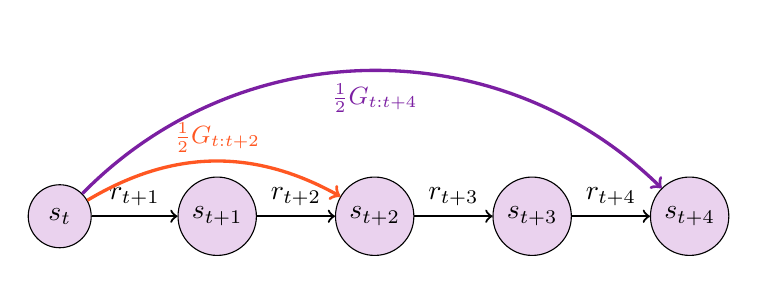
\begin{tikzpicture}[
            state/.style={circle, draw, minimum size=0.8cm, fill=etlight!30},
            arrow/.style={->, thick},
            label/.style={font=\small}
        ]
            % States
            \node[state] (s0) at (0,0) {$s_t$};
            \node[state] (s1) at (2,0) {$s_{t+1}$};
            \node[state] (s2) at (4,0) {$s_{t+2}$};
            \node[state] (s3) at (6,0) {$s_{t+3}$};
            \node[state] (s4) at (8,0) {$s_{t+4}$};

            % Transitions
            \draw[arrow] (s0) -- (s1) node[midway, above] {$r_{t+1}$};
            \draw[arrow] (s1) -- (s2) node[midway, above] {$r_{t+2}$};
            \draw[arrow] (s2) -- (s3) node[midway, above] {$r_{t+3}$};
            \draw[arrow] (s3) -- (s4) node[midway, above] {$r_{t+4}$};

            % 2-step return arrow
            \draw[->, very thick, etaccent] (s0) to[bend left=30] (s2);
            \node[label, etaccent] at (2,1) {$\frac{1}{2}G_{t:t+2}$};

            % 4-step return arrow
            \draw[->, very thick, etmain] (s0) to[bend left=45] (s4);
            \node[label, etmain] at (4,1.5) {$\frac{1}{2}G_{t:t+4}$};

            % Combined target
            % \node[label, ettrace, font=\normalsize] at (10, 0) {Combined Target = $\frac{1}{2}G_{t:t+2} + \frac{1}{2}G_{t:t+4}$};
        \end{tikzpicture}
    \end{center}

    \begin{block}<2->{Limitation}
        Compound updates can only be computed when the \textcolor{eterror}{\textbf{longest component}} is complete.
    \end{block}
\end{frame}

\begin{frame}
    \frametitle{The $\lambda$-Return Definition}

    \begin{block}<1->{TD($\lambda$) Weighting Scheme}
        Weight each n-step return proportionally to $\lambda^{n-1}$, then normalize:
    \end{block}

    \begin{block}<2->{$\lambda$-Return Formula}
        \begin{equation}
            G^\lambda_t = (1-\lambda)\sum_{n=1}^\infty \lambda^{n-1}G_{t:t+n}
        \end{equation}
    \end{block}

    \begin{block}<3->{Key Properties}
        \begin{itemize}
            \item<3-> \textcolor{etlambda}{\textbf{Exponential decay}}: Weight fades by $\lambda$ with each additional step
            \item<4-> \textcolor{etvalue}{\textbf{Normalization}}: Factor $(1-\lambda)$ ensures weights sum to 1
            \item<5-> \textcolor{etmain}{\textbf{Special cases}}:
                \begin{itemize}
                    \item $\lambda = 0$: $G^\lambda_t = G_{t:t+1}$ (Pure TD)
                    \item $\lambda = 1$: $G^\lambda_t = G_t$ (Pure MC)
                \end{itemize}
        \end{itemize}
        \end{block}
\end{frame}

\begin{frame}
    \frametitle{Visualizing $\lambda$-Returns}

    \begin{center}
        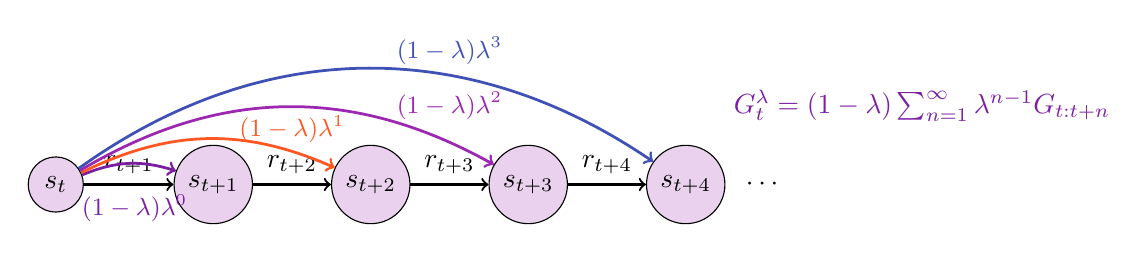
\begin{tikzpicture}[
            state/.style={circle, draw, minimum size=0.7cm, fill=etlight!30},
            arrow/.style={->, thick},
            label/.style={font=\small}
        ]
            % States
            \node[state] (s0) at (0,0) {$s_t$};
            \node[state] (s1) at (2,0) {$s_{t+1}$};
            \node[state] (s2) at (4,0) {$s_{t+2}$};
            \node[state] (s3) at (6,0) {$s_{t+3}$};
            \node[state] (s4) at (8,0) {$s_{t+4}$};
            \node at (9,0) {$\cdots$};

            % Transitions
            \draw[arrow] (s0) -- (s1) node[midway, above] {$r_{t+1}$};
            \draw[arrow] (s1) -- (s2) node[midway, above] {$r_{t+2}$};
            \draw[arrow] (s2) -- (s3) node[midway, above] {$r_{t+3}$};
            \draw[arrow] (s3) -- (s4) node[midway, above] {$r_{t+4}$};

            % 1-step return (thickest)
            \draw[->, line width=1pt, etmain] (s0) to[bend left=20] (s1);
            \node[label, etmain] at (1,-0.3) {$(1-\lambda)\lambda^0$};

            % 2-step return
            \draw[->, line width=1pt, etaccent] (s0) to[bend left=25] (s2);
            \node[label, etaccent] at (3,0.7) {$(1-\lambda)\lambda^1$};

            % 3-step return
            \draw[->, line width=1pt, ettrace] (s0) to[bend left=30] (s3);
            \node[label, ettrace] at (5,1) {$(1-\lambda)\lambda^2$};

            % 4-step return (thinnest)
            \draw[->, line width=1pt, etsecondary] (s0) to[bend left=35] (s4);
            \node[label, etsecondary] at (5,1.7) {$(1-\lambda)\lambda^3$};

            % Lambda-return formula
            \node[label, etmain, font=\normalsize] at (11,1) {$G^\lambda_t = (1-\lambda)\sum_{n=1}^\infty \lambda^{n-1}G_{t:t+n}$};
        \end{tikzpicture}
    \end{center}

    \begin{block}<1->{Understanding the Diagram}
        \begin{itemize}
            \item<1-> Each arrow represents an n-step return
            \item<3-> Longer returns have exponentially smaller weights
        \end{itemize}
    \end{block}

    \begin{block}<4->{Activity}
        \textcolor{ettrace}{\textbf{Why do we normalize by $(1-\lambda)$? What happens after terminal states?}}
    \end{block}
\end{frame}

\begin{frame}
    \frametitle{Activity Solution}

    \begin{block}<1->{Why Normalize by $(1-\lambda)$?}
        Need weights to sum to 1 for a proper average:
        \begin{align}
            \sum_{n=1}^\infty \lambda^{n-1} &= \frac{1}{1-\lambda}
        \end{align}
        So $(1-\lambda) \times \frac{1}{1-\lambda} = 1$
    \end{block}

    \begin{block}<2->{After Terminal States}
        \begin{itemize}
            \item<2-> After terminal state, all n-step returns equal the conventional return $G_t$
            \item<3-> $G_{t:t+n} = G_t$ for all $n \geq T-t$
            \item<4-> Therefore: $G^\lambda_t = G_t$ (becomes pure Monte Carlo)
        \end{itemize}
    \end{block}

    \begin{block}<5->{Key Insight}
        \textcolor{etmain}{\textbf{$\lambda$-returns automatically adapt}}: TD-like during episode, MC-like at termination!
    \end{block}
\end{frame}

% Section: TD Lambda
\section{TD($\lambda$) Algorithm}

\subsection{The Eligibility Trace Mechanism}

\begin{frame}
    \frametitle{TD($\lambda$): The Classic Algorithm}

    \begin{block}<1->{Historical Significance}
        \textcolor{etmain}{\textbf{TD($\lambda$)}} is one of the oldest and most widely used algorithms in reinforcement learning.
    \end{block}

    \begin{block}<2->{The Eligibility Trace Vector}
        \begin{itemize}
            \item<2-> $\mathbf{z}_t \in \mathbb{R}^d$ has same dimensions as weight vector $\mathbf{w}_t$
            \item<3-> Initialized to zero at episode start: $\mathbf{z}_0 = \mathbf{0}$
            \item<4-> Updated at each time step with two components:
                \begin{itemize}
                    \item<5-> \textcolor{ettrace}{\textbf{Decay}}: Previous traces fade by $\gamma\lambda$
                    \item<6-> \textcolor{etaccent}{\textbf{Increment}}: Add current state's feature gradient
                \end{itemize}
        \end{itemize}
        \end{block}

    \begin{block}<7->{Trace Update Equation}
        \begin{align}
            \mathbf{z}_0 &= \mathbf{0}\\
            \mathbf{z}_t &= \gamma\lambda\mathbf{z}_{t-1} + \nabla\hat{v}(s_t,\mathbf{w}_t)
        \end{align}
    \end{block}
\end{frame}

\begin{frame}
    \frametitle{Understanding Eligibility Traces}

    \begin{block}<1->{What Do Traces Track?}
        Eligibility traces keep track of which components of $\mathbf{w}$ have contributed to \textcolor{etvalue}{\textbf{recent}} state valuations.
    \end{block}

    \begin{block}<2->{Definition of "Recent"}
        \begin{itemize}
            \item<2-> "Recency" is defined by the product $\gamma\lambda$
            \item<3-> \textcolor{etlambda}{$\lambda = 0$}: Only current state eligible
            \item<4-> \textcolor{etlambda}{$\lambda = 1$}: All visited states remain eligible
            \item<5-> \textcolor{etlambda}{$0 < \lambda < 1$}: Exponential decay of eligibility
        \end{itemize}
    \end{block}

    \begin{block}<6->{Eligibility for Learning}
        \begin{itemize}
            \item<6-> Traces indicate \textcolor{ettrace}{\textbf{eligibility}} of each weight component
            \item<7-> Higher trace $\Rightarrow$ more eligible for learning changes
            \item<8-> Based on current TD error $\delta_t$
        \end{itemize}
    \end{block}
\end{frame}

\begin{frame}
    \frametitle{TD($\lambda$) Update Rules}

    \begin{block}<1->{TD Error (Same as TD(0))}
        \begin{equation}
            \delta_t = r_{t+1} + \gamma\hat{v}(s_{t+1},\mathbf{w}_t) - \hat{v}(s_t,\mathbf{w}_t)
        \end{equation}
        \end{block}

    \begin{block}<2->{Weight Update (New!)}
        \begin{equation}
            \mathbf{w}_{t+1} = \mathbf{w}_t + \alpha\delta_t\mathbf{z}_t
        \end{equation}
        \end{block}

    \begin{block}<3->{Key Insight}
        \begin{itemize}
            \item<3-> \textcolor{eterror}{\textbf{Single TD error}} $\delta_t$ affects multiple weight components
            \item<4-> Each component updated proportional to its \textcolor{ettrace}{\textbf{eligibility}}
            \item<5-> Recently visited states get larger updates
        \end{itemize}
        \end{block}

    \begin{block}<6->{Comparison to TD(0)}
        \begin{itemize}
            \item<6-> \textbf{TD(0)}: Only current state updated
            \item<7-> \textbf{TD($\lambda$)}: All recently visited states updated
        \end{itemize}
    \end{block}
\end{frame}

\begin{frame}
    \frametitle{TD($\lambda$) Algorithm}

    \begin{center}
        \includegraphics[width=0.5\textwidth]{../lectures/rl/eligibility-traces/td-lambda.png}
    \end{center}
\end{frame}

\begin{frame}
    \frametitle{The Backward View Mechanism}

    \begin{block}<1->{Backward Perspective}
        \textcolor{etbackward}{\textbf{Backward view}}: Each update depends on current TD error combined with eligibility traces of past events.
    \end{block}

    \begin{center}
        \includegraphics[width=0.8\textwidth]{../lectures/rl/eligibility-traces/backward-mechanism.png}
    \end{center}

    \begin{block}<2->{How It Works}
        \begin{itemize}
            \item<2-> Current reward/error propagates \textcolor{etbackward}{\textbf{backward}} to eligible states
            \item<3-> More recently visited states get more credit
            \item<4-> Exponential decay ensures finite computational cost
        \end{itemize}
    \end{block}
\end{frame}

% Section: SARSA Lambda
\section{SARSA($\lambda$)}

\subsection{Extending to Action Values}

\begin{frame}
    \frametitle{From State Values to Action Values}

    \begin{block}<1->{Moving to Control}
        We want to learn approximate action values $\hat{q}(s,a,\mathbf{w})$ instead of state values.
    \end{block}

    \begin{block}<2->{Modified Components}
        \textbf{Weight Update (Same Pattern):}
        \begin{equation}
            \mathbf{w}_{t+1} = \mathbf{w}_t + \alpha\delta_t\mathbf{z}_t
        \end{equation}

        \textbf{TD Error (For Action Values):}
        \begin{equation}
            \delta_t = r_{t+1} + \gamma\hat{q}(s_{t+1},a_{t+1},\mathbf{w}_t) - \hat{q}(s_t,a_t,\mathbf{w}_t)
        \end{equation}

        \textbf{Eligibility Trace (For Action Values):}
        \begin{align}
            \mathbf{z}_0 &= \mathbf{0}\\
            \mathbf{z}_t &= \gamma\lambda\mathbf{z}_{t-1} + \nabla\hat{q}(s_t, a_t, \mathbf{w}_t)
        \end{align}
    \end{block}
\end{frame}

\begin{frame}
    \frametitle{SARSA($\lambda$) Algorithm}

    \begin{center}
        \includegraphics[width=0.5\textwidth]{../lectures/rl/eligibility-traces/sarsa-lambda.png}
    \end{center}
\end{frame}

\begin{frame}
    \frametitle{Understanding SARSA($\lambda$)}

    \begin{block}<1->{Key Differences from SARSA(0)}
        \begin{itemize}
            \item<1-> \textbf{SARSA(0)}: Only current $(s,a)$ pair updated
            \item<2-> \textbf{SARSA($\lambda$)}: All recently visited $(s,a)$ pairs updated
            \item<3-> \textcolor{ettrace}{\textbf{Eligibility traces}} remember which actions were taken recently
        \end{itemize}
    \end{block}

    \begin{block}<4->{Benefits}
        \begin{itemize}
            \item<4-> \textcolor{eteval}{\textbf{Faster learning}}: Information propagates to multiple state-action pairs
            \item<5-> \textcolor{etbackward}{\textbf{Better credit assignment}}: Past actions get immediate feedback
            \item<6-> \textcolor{etvalue}{\textbf{Sample efficiency}}: Each experience updates many values
        \end{itemize}
    \end{block}

    \begin{block}<7->{Activity}
        \textcolor{etactivity}{\textbf{Read through the SARSA($\lambda$) pseudocode and identify the key steps.}}
    \end{block}
\end{frame}

% Section: Advanced Topics
\section{Advanced Topics}

\subsection{Replacing vs Accumulating Traces}

\begin{frame}
    \frametitle{Types of Eligibility Traces}

    \begin{block}<1->{Accumulating Traces (What We've Seen)}
        \begin{equation}
            \mathbf{z}_t = \gamma\lambda\mathbf{z}_{t-1} + \nabla\hat{q}(s_t, a_t, \mathbf{w}_t)
        \end{equation}
        Traces \textcolor{etaccent}{\textbf{accumulate}} each time a state-action pair is revisited.
    \end{block}

    \begin{block}<2->{Replacing Traces}
        \begin{equation}
            z_t(s,a) = \begin{cases}
                \gamma\lambda z_{t-1}(s,a) & \text{if } (s,a) \neq (s_t,a_t)\\
                1 & \text{if } (s,a) = (s_t,a_t)
            \end{cases}
        \end{equation}
        Traces are \textcolor{eterror}{\textbf{reset to 1}} when a state-action pair is revisited.
    \end{block}

    \begin{block}<3->{When to Use Each}
        \begin{itemize}
            \item<3-> \textbf{Accumulating}: Function approximation, continuous spaces
            \item<4-> \textbf{Replacing}: Tabular methods, discrete spaces
            \item<5-> \textbf{Replacing} often works better in practice for tabular methods
        \end{itemize}
    \end{block}
\end{frame}

\begin{frame}
    \frametitle{Implementation Considerations}

    \begin{block}<1->{Computational Efficiency}
        \begin{itemize}
            \item<1-> \textcolor{etvalue}{\textbf{Sparse updates}}: Only update non-zero traces
            \item<2-> \textcolor{ettrace}{\textbf{Trace cutoff}}: Set traces to zero when below threshold
            \item<3-> \textcolor{etlambda}{\textbf{Memory management}}: Traces can grow large in long episodes
        \end{itemize}
    \end{block}

    \begin{block}<4->{Parameter Selection}
        \begin{itemize}
            \item<4-> \textcolor{etlambda}{$\lambda$}: Higher values $\Rightarrow$ more like Monte Carlo
            \item<5-> \textcolor{etaccent}{$\alpha$}: Learning rate may need adjustment with $\lambda$
            \item<6-> \textcolor{etmain}{$\gamma$}: Affects both discounting and trace decay
        \end{itemize}
    \end{block}

    \begin{block}<7->{Practical Tips}
        \begin{itemize}
            \item<7-> Start with $\lambda = 0.9$ as a default
            \item<8-> Use replacing traces for tabular methods
            \item<9-> Monitor trace magnitudes to ensure they're decaying properly
        \end{itemize}
    \end{block}
\end{frame}

\subsection{True Online TD($\lambda$)}

\begin{frame}
    \frametitle{Beyond Basic Eligibility Traces}

    \begin{block}<1->{Limitation of Semi-Gradient Methods}
        The TD($\lambda$) we've seen is a \textcolor{eterror}{\textbf{semi-gradient}} method:
        \begin{itemize}
            \item<1-> Updates don't account for changing targets
            \item<2-> Not equivalent to gradient descent on any objective function
            \item<3-> Can be unstable with function approximation
        \end{itemize}
    \end{block}

    \begin{block}<4->{True Online TD($\lambda$)}
        \begin{itemize}
            \item<4-> \textcolor{etmain}{\textbf{True gradient}} method for $\lambda$-return objective
            \item<5-> More complex update rules but better theoretical properties
            \item<6-> Often performs better in practice with function approximation
        \end{itemize}
    \end{block}

    \begin{block}<7->{When It Matters}
        \begin{itemize}
            \item<7-> \textbf{Function approximation}: Neural networks, linear functions
            \item<8-> \textbf{Stability concerns}: When basic TD($\lambda$) diverges
            \item<9-> \textbf{Theoretical guarantees}: When convergence proofs are needed
        \end{itemize}
    \end{block}
\end{frame}

% Section: Applications and Comparisons
\section{Applications and Comparisons}

\subsection{Eligibility Traces in Practice}

\begin{frame}
    \frametitle{Real-World Applications}

    \begin{block}<1->{Game Playing}
        \begin{itemize}
            \item<1-> \textcolor{etmain}{\textbf{TD-Gammon}}: Used TD($\lambda$) to achieve superhuman backgammon play
            \item<2-> \textcolor{etaccent}{\textbf{Chess engines}}: Temporal difference learning with eligibility traces
            \item<3-> \textcolor{etvalue}{\textbf{Go programs}}: Combined with Monte Carlo Tree Search
        \end{itemize}
    \end{block}

    \begin{block}<4->{Robotics}
        \begin{itemize}
            \item<4-> \textbf{Robot navigation}: Learning from delayed rewards
            \item<5-> \textbf{Manipulation}: Credit assignment for complex motor skills
            \item<6-> \textbf{Multi-agent systems}: Coordinated learning with traces
        \end{itemize}
    \end{block}

    \begin{block}<7->{Finance and Control}
        \begin{itemize}
            \item<7-> \textbf{Portfolio optimization}: Learning from market feedback
            \item<8-> \textbf{Process control}: Industrial control systems
            \item<9-> \textbf{Resource allocation}: Dynamic pricing and scheduling
        \end{itemize}
    \end{block}
\end{frame}

\begin{frame}
    \frametitle{Performance Characteristics}

    \begin{block}<1->{Learning Speed}
        \begin{center}
        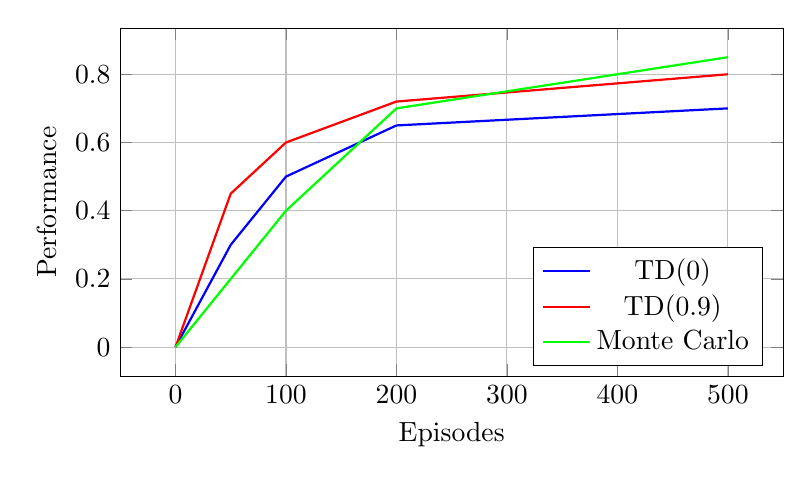
\begin{tikzpicture}
            \begin{axis}[
                xlabel={Episodes},
                ylabel={Performance},
                width=10cm,
                height=6cm,
                legend pos=south east,
                grid=major
            ]
            \addplot[blue, thick] coordinates {(0,0) (50,0.3) (100,0.5) (200,0.65) (500,0.7)};
            \addlegendentry{TD(0)}
            \addplot[red, thick] coordinates {(0,0) (50,0.45) (100,0.6) (200,0.72) (500,0.8)};
            \addlegendentry{TD(0.9)}
            \addplot[green, thick] coordinates {(0,0) (50,0.2) (100,0.4) (200,0.7) (500,0.85)};
            \addlegendentry{Monte Carlo}
            \end{axis}
        \end{tikzpicture}
        \end{center}
    \end{block}

    \begin{block}<2->{Key Observations}
        \begin{itemize}
            \item<2-> \textcolor{etlambda}{\textbf{TD($\lambda$)}} often converges faster than pure TD or MC
            \item<3-> \textcolor{etvalue}{\textbf{Intermediate $\lambda$}} values (0.8-0.95) often optimal
            \item<4-> \textcolor{ettrace}{\textbf{Problem-dependent}}: Best $\lambda$ varies by domain
        \end{itemize}
    \end{block}
\end{frame}

\subsection{Summary and Extensions}

\begin{frame}
    \frametitle{Key Takeaways}

    \begin{block}<1->{What We've Learned}
        \begin{itemize}
            \item<1-> \textcolor{etmain}{\textbf{Eligibility traces}} unify Monte Carlo and TD methods
            \item<2-> \textcolor{ettrace}{\textbf{$\lambda$-parameter}} controls the trade-off between bias and variance
            \item<3-> \textcolor{etbackward}{\textbf{Backward view}}: Efficient credit assignment mechanism
            \item<4-> \textcolor{etvalue}{\textbf{Computational efficiency}}: Single error updates multiple states
        \end{itemize}
    \end{block}

    \begin{block}<5->{Algorithm Spectrum}
        \begin{center}
        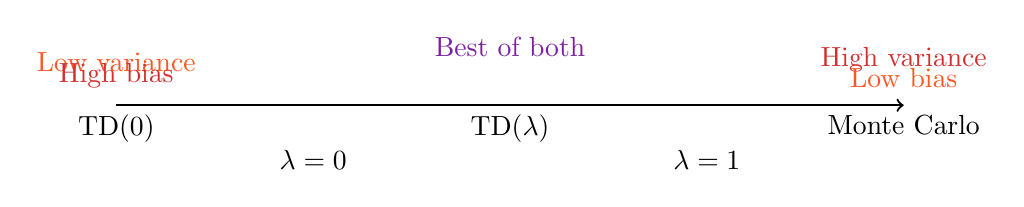
\begin{tikzpicture}
            \draw[thick,->] (0,0) -- (10,0);
            \node[below] at (0,0) {TD(0)};
            \node[below] at (5,0) {TD($\lambda$)};
            \node[below] at (10,0) {Monte Carlo};

            \node[above] at (0,0.3) {\textcolor{etaccent}{Low variance}};
            \node[above] at (0,0.1) {\textcolor{eterror}{High bias}};

            \node[above] at (10,0.3) {\textcolor{eterror}{High variance}};
            \node[above] at (10,0.1) {\textcolor{etaccent}{Low bias}};

            \node[above] at (5,0.5) {\textcolor{etmain}{Best of both}};

            \node at (2.5,-0.7) {$\lambda = 0$};
            \node at (7.5,-0.7) {$\lambda = 1$};
        \end{tikzpicture}
        \end{center}
    \end{block}
\end{frame}

\begin{frame}
    \frametitle{Extensions and Modern Developments}

    \begin{block}<1->{Function Approximation}
        \begin{itemize}
            \item<1-> \textcolor{etmain}{\textbf{Neural networks}}: Deep RL with eligibility traces
            \item<2-> \textcolor{etaccent}{\textbf{Linear function approximation}}: Convergence guarantees
            \item<3-> \textcolor{ettrace}{\textbf{Feature selection}}: Sparse eligibility traces
        \end{itemize}
    \end{block}

    \begin{block}<4->{Policy Methods}
        \begin{itemize}
            \item<4-> \textbf{Actor-Critic($\lambda$)}: Traces for both value and policy
            \item<5-> \textbf{Policy gradient traces}: Eligibility traces for policy parameters
            \item<6-> \textbf{Natural gradients}: Combined with eligibility traces
        \end{itemize}
    \end{block}

    \begin{block}<7->{Modern Algorithms}
        \begin{itemize}
            \item<7-> \textbf{Retrace($\lambda$)}: Off-policy traces with importance sampling
            \item<8-> \textbf{Impala}: Distributed RL with traces
            \item<9-> \textbf{Rainbow DQN}: Modern deep RL incorporating trace-like mechanisms
        \end{itemize}
    \end{block}
\end{frame}

\begin{frame}
    \frametitle{Looking Forward}

    \begin{block}<1->{Next Steps in Your RL Journey}
        \begin{itemize}
            \item<1-> \textcolor{eteval}{\textbf{Function approximation}}: Linear and non-linear methods
            \item<2-> \textcolor{etpolicy}{\textbf{Policy gradient methods}}: Direct policy optimization
            \item<3-> \textcolor{etvalue}{\textbf{Deep reinforcement learning}}: Neural network function approximation
            \item<4-> \textcolor{etmain}{\textbf{Advanced topics}}: Multi-agent RL, hierarchical RL, meta-learning
        \end{itemize}
    \end{block}

    \begin{block}<5->{Key Insight}
        \textcolor{ettrace}{\textbf{Eligibility traces}} provide the foundation for understanding how credit assignment works in reinforcement learning - a crucial concept that appears in many modern algorithms!
    \end{block}

    \begin{block}<6->{Final Thought}
        \begin{center}
            \textcolor{etmain}{\textit{"The best way to understand eligibility traces is to implement and experiment with them yourself."}}
        \end{center}
    \end{block}
\end{frame}

\end{document}
